Nous avons vu deux manières de résoudre l'équation de Poisson avec conditions aux bords de Dirichlet. Nous allons maintenant présenter une troisième méthode  : \\
\begin{center}
Le méthode de Douglas
\end{center}
Soit $I$, l'image à retrouver : 
%%%%%%%%%%%%%%%%%%%%%%%%%%%%%%%%%%%%%%%%
\subsubsection{D'un problème avec contraintes...}
Remarquons que le problème initial est un problème d'optimisation avec contraintes. En effet, nous voulons minimiser $\int_\Omega ||\nabla I-\nabla S||^2$. Avec la contrainte suivante : $I = T$ en dehors du domaine. \\
Ce problème d'optimisation peut donc être résolu à l'aide de différents algorithmes, mais avant ça, transformons-le en un problème sans contraintes. 

\subsubsection{... À un problème sans contraintes}
En utilisant des fonctions de pénalisation nous remarquons aisément que ce problème peut être ramené à un problème sans contraintes. Réécrivons donc celui-ci 
\begin{equation*}
\begin{aligned}{}
    min \int_\Omega ||\nabla I - \nabla S||^2 + \mathbb{1} _{D \backslash \Omega } (I) \\
    \end{aligned}
\end{equation*}{}
avec 
\begin{equation*}
\mathbb{1}_{ D \backslash \Omega }(I) =
	\left\{
	\begin{aligned}{}
	0 \ si\  I \in T \backslash \Omega \\
	+ \infty \ sinon
    \end{aligned}
    \right.
\end{equation*}{}
Dans la suite nous noterons $K = T\backslash \Omega$. K représente donc l'ensemble des images dont les pixels situés en dehors du domaine$\Omega$, coïncident avec T.\\

Nous avons bien équivalence entre notre problème sans contraintes et le problème (1). En effet, si I $\in K$, alors l'indicatrice vaut 0 et nous devons juste résoudre $min \int_\Omega ||\nabla I - \nabla S||^2 $. Si au contraire $I \notin K$, alors nous devons minimiser quelque chose qui vaut plus $+\infty$. Le minimum n'existe pas, il n'y a pas de solutions.\\
 En effet, l'image I ne coïncide pas avec T à l'extérieur de $\Omega$,  la condition I = T en dehors du domaine n'étant pas respectée, le problème n'a pas de solution. \\
 Ce problème sans contraintes, traduit bien celui avec contraintes. Nous pouvons donc essayer de résoudre celui-ci, numériquement. Afin d'être sûrs que le minimum existe, nous montrerons dans la suite que cette fonction est bien convexe. 
 Par commodité, nous noterons dans la suite : 
 \begin{equation*}
 \begin{aligned}
 F(I) &=   \int_\Omega ||\nabla I - \nabla S||^2 + \mathbb{1} _{T\backslash \Omega } (I) \\
 & = f(I)+ g(I)
 \end{aligned}
 \end{equation*}
\subsubsection{La convexité...}
Montrons que K est convexe. 
Soit u et v deux images appartenant à K, alors, les pixels de u et de v, se situant à l'extérieur de $\Omega$, coïncident avec les pixels de T. \\
Considérons maintenant une nouvelle image : 
\begin{center}
$M = \lambda u+(1-\lambda)v$
\end{center}
Les pixels de u et v coïncidant avec ceux de T à l'extérieur, nous pouvons réécrire les pixels de $M$ de la manière suivante. \\

\begin{equation*} 
M (i,j) = 
\left\{
\begin{aligned}
\lambda u(i,j) +(1-\lambda) v(i,j), \ \ (i,j) \in \Omega\\
\lambda T(i,j) +(1-\lambda )T(i,j))  \ \ (i,j)\notin \Omega
\end{aligned}
\right.
\end{equation*}
Ainsi, pour $(i,j) \notin \Omega$ : \\
\begin{center}
$M_{i,j} = \lambda T_{i,j}+(1-\lambda) T_{i,j} = T_{i,j}$
\end{center}
Ainsi, les pixels de M n'appartenant pas à $\Omega$, coïncident avec T.M appartient bien à K. Et K est donc convexe.\\
K étant convexe, et non vide, (T en particulier appartient à K), alors la fonction $\mathbb{1}_K(I)$ est convexe. \\
Enfin montrons la convexité de $||\nabla I-\nabla S||^2$.
La norme étant une fonction convexe et croissante, alors la fonction : $||.||^2$ est elle aussi convexe. 
Nous avons donc $f et g$, convexes, ainsi, la fonction $F =f+g$ est elle aussi convexe. Elle admet donc un minimum. Nous pouvons ainsi résoudre numériquement ce problème.
\subsubsection{... Pour utiliser l'algorithme de Douglas...}
L'algorithme que nous allons utiliser est l'algorithme de Douglas-Rachford. Cet algorithme permet d'approcher le minimum  d'une fonction $F = f+g$, f et g étant des fonctions convexes, comme montré dans la partie précédente, nous pouvons utiliser cet algorithme.
\paragraph{L'algorithme}
À chaque itération, sont calculés : 
\begin{center}
$x_{k+1} = prox_f(y_k)$\\
$y_{k+1} = y_k+prox_g(2x_x{k+1}-y_k)-x_{k+1}$
\end{center}{}
Il est donc nécessaire de calculer les opérateurs proximaux respectifs de $f$ et $g$. 
\subsubsection{... Avec les opérateurs proximaux ...}
Un opérateur proximal est défini comme suit : 
\begin{center}
\begin{equation*}
\begin{aligned}
prox_f(x) = argmin_u \left\{ \frac{||u-x||^2}{2}+ f(u)\right\}
\end{aligned}
\end{equation*}
\end{center}
\paragraph{Opérateur proximal de f}
\begin{equation*}
prox_f(x) = argmin_u\left\{\frac{||u-x||^2}{2}+||\nabla u -\nabla S ||^2 \right\}
\end{equation*}
Afin de faciliter les notations notons :
\begin{equation*}
h(u) = \frac{||u-x||^2}{2}+||\nabla u -\nabla S ||^2
\end{equation*} 
Nous cherchons donc 
\begin{center}
$argmin_u h(u)$
\end{center}
ie. u qui minimise la fonction h, autrement dit, un u qui annule le gradient de h.\\
En utilisant Taylor Young, 

\begin{equation*}
\begin{aligned}
h(u+k) -h(u) &= \frac{||u+k-x||^2}{2}+||\nabla  (u+k) -\nabla S ||^2- \frac{||u-x||^2}{2}-||\nabla u -\nabla S ||^2\\
& = \frac{||k||^2+2\left<u-x,k\right>}{2}+||\nabla k||^2+2\left<\nabla u-\nabla S, \nabla k\right>\\
& = O(||k||^2)+\left<u-x,k\right>-2\left<div(\nabla u-\nabla S), k\right>\\
& = \left<u-x-2div(\nabla u-\nabla S), k\right>\\
\end{aligned}
\end{equation*}
Nous obtenons le gradient de h.
\begin{equation*}
\begin{aligned}
\nabla h(u) &= u-x-2div(\nabla u - \nabla S)\\
& = u-x-2(\Delta u -\Delta S)
\end{aligned}
\end{equation*}
En résolvant $\nabla h(u) = 0$, nous pourrons trouver  : $prox_f(x) $. \\	
	\begin{equation*}
		\begin{aligned}
		\nabla h(u) &= 0\\
		u-x-2(\Delta u -\Delta S) & =0\\
		u-2\Delta u = x-2\Delta S
		\end{aligned}
\end{equation*}
Afin de trouver u, nous utiliserons la méthode des différences finies. En discrétisant le laplacien de u, comme nous l'avons vu dans la section (1) : 
\begin{equation*}
 -2u(x+1,y) -2 u(x-1,y)-2u(x,y+1) -2 u(x,y-1) +9\times u(x,y) =  y_k-  2\Delta S(x,y)
\end{equation*}
En mettant ce système sous forme matricielle nous pourrons approcher u en faisant une inversion matricielle. 
Nous pouvons donc numériquement approcher $prox_f(x)$.

\paragraph{Opérateur proximal de g}
g étant la fonction indicatrice suivante : 
\begin{equation*}
\mathbb{1}_{ D \backslash \Omega }(I) =
	\left\{
	\begin{aligned}{}
	0 \ si\  I \in T \backslash \Omega \\
	+ \infty \ sinon
    \end{aligned}
    \right.
\end{equation*}{}
Nous avons donc 
\begin{equation*}
prox_g(x) =  argmin_u\left\{\frac{||u-x||^2}{2}+ \mathbb{1}_K(u)\right\}
\end{equation*}
Nous savons que $prox_g(x)$ existe puisque la fonction g est convexe et la fonction norme est elle aussi convexe.
Notons $h(u) = \frac{||u-x||^2}{2}+ \mathbb{1}_K(u)$ 
Comme nous l'avons cette fonction n'admet un minimum que si $u \in K$. Supposons donc $u \in K$. Alors chercher $argmin_u \left\{h(u)\right\}$ est équivalent à chercher $argmin_{u\in K} \left\{\frac{||u-x||^2}{2}\right\}$.\\
Dans notre cas, u $prox_g(x) = L$.
L étant une image appartenant à K, et dont les pixels à l'intérieur de $\Omega$ coïncident avec x.\\
\subsubsection{Convergence de l'algorithme vers la solution}
\begin{figure}[!htb]
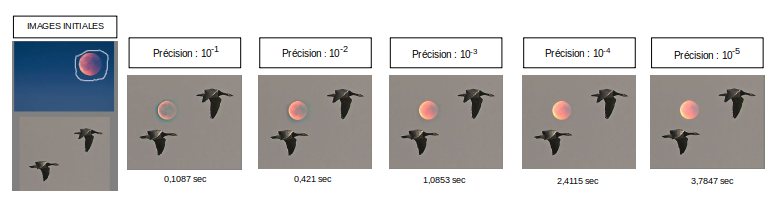
\includegraphics[scale=0.6]{Images/Resultats/conv1.png}
\caption{Convergence de l'algorithme vers la solution}
\end{figure}
\begin{figure}[!htb]
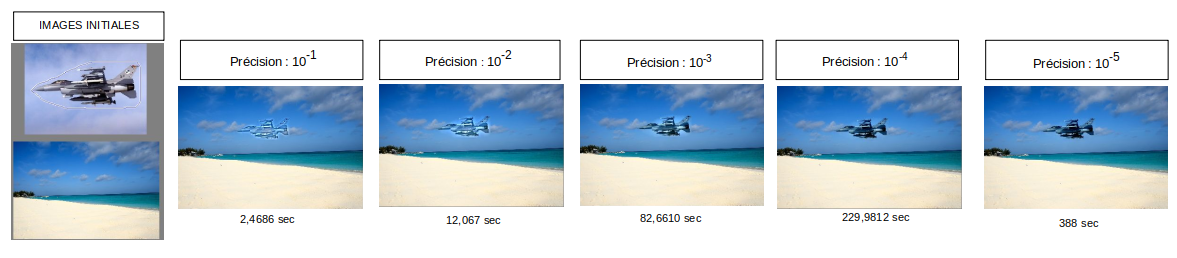
\includegraphics[scale=0.4]{Images/Resultats/conv2.png}
\caption{Convergence de l'algorithme vers la solution}
\end{figure}
L'algorithme de Douglas converge bien vers une solution I qui résout le problème initial.
\subsubsection{Temps et coût de l'algorithme}
L'algorithme semble être très efficace, malheureusement en termes de temps de calcul, il est très long. Nous ferons dans la prochaine partie un tableau comparatif des temps de calculs effectués sur des images de tailles différentes.\\
Nous avons considérablement amélioré  le temps de calcul de l'algorithme de Douglas-Rachford, en utilisant l'algorithme du gradient conjugué, afin d'inverser la matrice de l'opérateur proximal de f. Malgré tout, l'algorithme est encore lent sur de grandes images. Nous choisissons une précision de $10^{-5}$, afin d'avoir des résultats convenables et comparables à ceux obtenus avec les méthodes précédentes. Le nombre d'itérations de l'algorithme devient alors très important, car il semble converger plus lentement à partir de $10^-3$, ce qui augmente considérablement le temps de calcul.\\
Nous avons amélioré les temps de calculs en appliquant une méthode de sur-relaxation sur l'algorithme de Douglas-Rachford, avec un $\rho  =1.85$.A chaque itération nous calculons donc :
\begin{center} 
\begin{itemize}
\item $x_{k+1} = prox_f(y_k)$
\item $y_{k+1} = y_k+\rho_k(prox_g(2x_{k+1}-y_k)-x_{k+1})$
\end{itemize}
\end{center}
($1<\rho<2$).\\
Cependant, le temps de calcul est encore élevé sur de grandes images.
Afin de réduire ce temps de calcul il faudrait donc que l'algorithme converge encore plus rapidement vers la solution. Pour cela, nous proposons d'augmenter l'ordre de discrétisation du Laplacien. Nous étions jusqu'à présent d'ordre 2, peut -être faudrait-il augmenter cette précision jusqu'à l'ordre 8.
\subsection{Tableau comparatif}
\begin{tabular}{|c|c|c|c|c|c|}
\hline
Taille de l'image S & Taille de l'image T& Temps Douglas & \shortstack{Temps Douglas \\(R)} &\shortstack{Temps différences\\ finies} & Temps Fourier\\
\hline
220 $\times$ 154 $\times$3 px & 304 $\times $252 $\times $3 px &  \shortstack{ 834 itérations\\ précision : 5$\times 10^{-5}$\\3.799 secondes} &\shortstack{ 547 itérations\\
précision : $5 \times 10^{-5}$\\ 2.2233 secondes}&  0.335 secondes & 0.355 secondes \\

\hline
304 $\times$ 252 $\times$3 px & 770$\times$844 $\times $3 px & \shortstack{ 1591 itérations\\ précision : 5$\times 10^{-5}$\\72.348 secondes} & \shortstack{ 1182 itérations\\
précision : $5 \times 10^{-5}$\\ 46.1067 secondes} & 0.797 secondes & 1.640 secondes \\
\hline
400 $\times$ 300 $\times$3 px & 1200$\times$800$\times $3 px & \shortstack{ 6224 itérations\\ précision : 5$\times 10^{-5}$\\440.886 secondes} &\shortstack{3884 itérations\\ précision : 5$\times 10^{-5}$\\205.8105 secondes} &1.05 secondes & 2.102 secondes \\
\hline
400 $\times$ 300 $\times$3 px & 614$\times$441$\times $3 px & \shortstack{ 5448 itérations\\ précision : 5$\times 10^{-5}$\\366.0.34 secondes}&\shortstack{4046 itérations\\ précision : 5$\times 10^{-5}$\\224.3881 secondes} & 0.877 secondes & 0.8576 secondes \\
\hline
220 $\times$ 154 $\times$3 px & 263$\times$192$\times $3 px & \shortstack{ 861 itérations\\ précision : 5$\times 10^{-5}$\\4.056 secondes} &\shortstack{510 itérations\\ précision : 5$\times 10^{-5}$\\2.3466 secondes}& 0.0892 secondes & 0.1754 secondes \\
\hline
\end{tabular}\\
Temps Douglas (R) est la méthode de surrelaxation couplée à la méthode de Douglas, $\rho = 1.89$. Nous remarquons qu'à l'aide de cette méthode, nous pouvons considérablement diminuer le nombre d'itérations de l'algorithme de Douglas-Rachford(il converge plus vite) et ainsi améliorer le temps de calcul de celui-ci. (jusqu'à t/2, sur de grandes images).
Les résultats que nous obtenons avec les différentes images sont à peu près similaires. Nous pouvons bien sûr raccourcir le temps de calcul de l'algorithme de Douglas-Rachford, en diminuant la précision. Mais dans ce cas, les résultats obtenus avec celui-ci sont moins bons, et non comparables avec ceux des deux autres méthodes. 
\section{Amélioration du collage}
Après avoir implémenté des "sliders", permettant de bouger la sélection sur l'image de fond, nous nous sommes compte que la sélection est parfois trop grande, et peut cacher des objets, ou choses importantes sur l'image de fond : 
\begin{figure}[!htb]
\centering
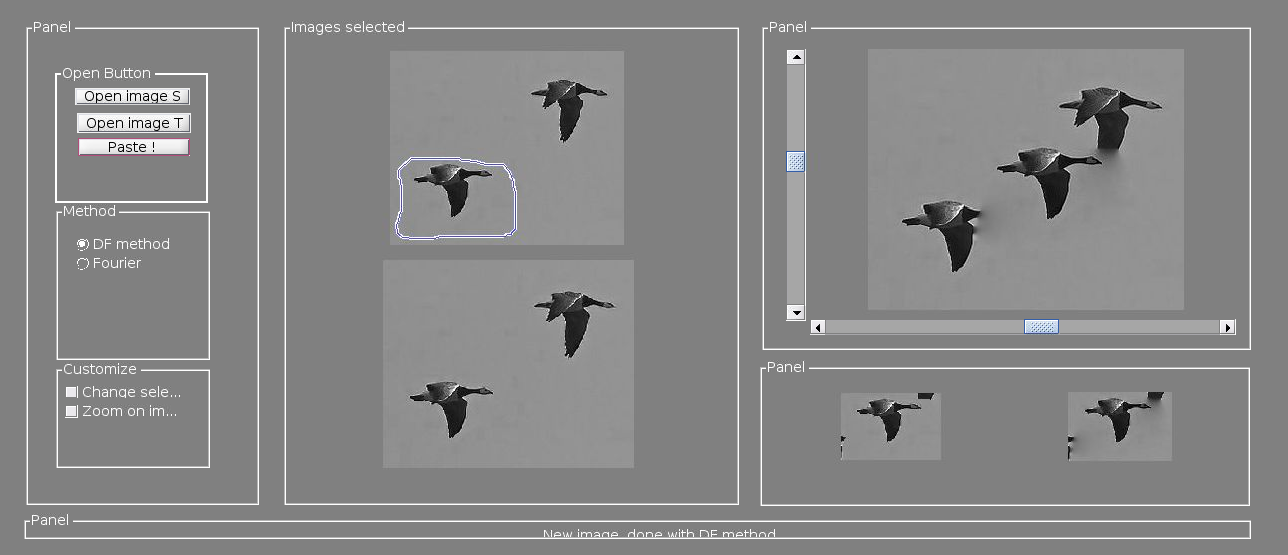
\includegraphics[scale=0.25]{Images/pb.png}
\caption{Problème rencontré}
\end{figure}
Nous voyons bien, ci-dessus, qu'en sélectionnant une grande zone autour de la lune dans l'image S,le collage cache effectivement l'oiseau, objet pourtant important de l'image T. Afin de résoudre ce problème, nous avons opté pour la comparaison des gradients dans chaque image. En effet, si le gradient de T est supérieur à celui de S, alors cela signifie que l'image T, possède un objet, ou un contour à cette position tandis que S ne possède rien d'important à la même position. Nous pouvons donc "réduire" la sélection et la modifier en ce pixel. Nous obtenons donc la figure suivante en utilisant cette propriété :
\begin{figure}[!h]
\centering
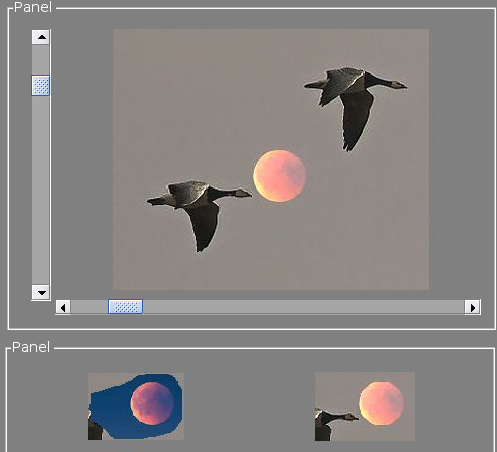
\includegraphics[scale=0.25]{Images/sol.png}
\caption{Problème résolu, algorithme utilisé : Différence Finie}
\end{figure}
\newpage
Cependant cette "amélioration" à ses limites, en effet, l'intérieur de la lune ne possède que très peu de variations et presque aucun contours, ainsi, si la lune se situait exactement sur la tête de l'oiseau, certains pixels à l'intérieur de celle-ci serait "supprimé" de la sélection, et ainsi, le résultat ne serait pas satisfaisant.
